\documentclass{beamer}
\mode<presentation>
{
  \usetheme{Warsaw}
  \definecolor{mcgarnet}{rgb}{0.38, 0, 0.08}
  \definecolor{mcgray}{rgb}{0.6, 0.6, 0.6}
  \setbeamercolor{structure}{fg=mcgarnet,bg=mcgray}
  %\setbeamercovered{transparent}
}


\usepackage[english]{babel}
\usepackage[latin1]{inputenc}
\usepackage{times}
\usepackage[T1]{fontenc}
\usepackage{tikz}
\usepackage{graphicx}

\newcommand{\imagesource}[1]{{\centering\hfill\break\hbox{\scriptsize Image Source:\thinspace{\small\itshape wikipedia.org}}\par}}

\title{Pointers and Terminal Control}


\author{Robert Lowe\\}

\institute[Maryville College] % (optional, but mostly needed)
{
  Division of Mathematics and Computer Science\\
  Maryville College
}

\date[]{}
\subject{}

\pgfdeclareimage[height=0.5cm]{university-logo}{images/Maryville-College}
\logo{\pgfuseimage{university-logo}}



\AtBeginSection[]
{
  \begin{frame}<beamer>{Outline}
    \tableofcontents[currentsection]
  \end{frame}
}


\begin{document}

\begin{frame}
  \titlepage
\end{frame}

\begin{frame}{Outline}
  \tableofcontents
\end{frame}


% Structuring a talk is a difficult task and the following structure
% may not be suitable. Here are some rules that apply for this
% solution: 

% - Exactly two or three sections (other than the summary).
% - At *most* three subsections per section.
% - Talk about 30s to 2min per frame. So there should be between about
%   15 and 30 frames, all told.

% - A conference audience is likely to know very little of what you
%   are going to talk about. So *simplify*!
% - In a 20min talk, getting the main ideas across is hard
%   enough. Leave out details, even if it means being less precise than
%   you think necessary.
% - If you omit details that are vital to the proof/implementation,
%   just say so once. Everybody will be happy with that.

\section{Pointers and References}
\begin{frame}
    \frametitle{A Primer on Computer Memory}
    \begin{columns}
        \column{0.6\textwidth}
        \begin{itemize}
            \item Memory is a large list.
            \item Typically, each BYTE of memory has an address.
            \item Memory can be read or written.
            \item In most computers, program code and data are in the same memory.
        \end{itemize}
        \column{0.4\textwidth}
        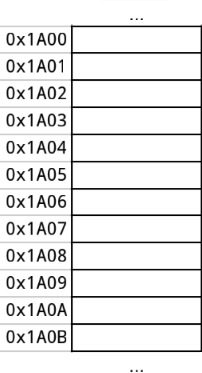
\includegraphics[height=0.75\textheight]{images/memlist}
    \end{columns}
\end{frame}

\begin{frame}
    \frametitle{The {\tt sizeof} operator}
    \begin{block}{Syntax}
        {\tt sizeof}({\em type})\par
        {\tt sizeof} {\em expression}
    \end{block}
    \begin{itemize}
        \item Each data type has a different size.
        \item {\tt sizeof} returns the size of the type or expression 
            which follows it.
        \item Example: {\tt sizeof(int)} returns 4 on our system.
        \item {\tt sizeof(double)} returns 8 on our system.
    \end{itemize}
\end{frame}

\begin{frame}
    \frametitle{How Variables are Stored in Memory}
    \begin{columns}
        \column{0.6\textwidth}
        \begin{itemize}
            \item Variables reside in memory.
            \item The compiler remembers the beginning 
                and size of each variable.
            \item Generated machine code refers to variables
                by their memory address.
            \item A variable is fully specified as:
                \begin{itemize}
                    \item A Memory Address
                    \item Size
                    \item Data 
                \end{itemize}
        \end{itemize}
        \column{0.4\textwidth}
        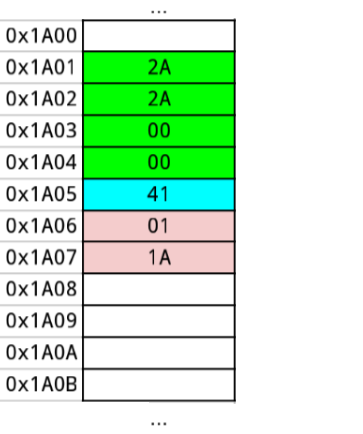
\includegraphics[height=0.60\textheight]{images/memdata}
    \end{columns}
\end{frame}

\begin{frame}
    \frametitle{Pointers}
    \begin{columns}
        \column{0.6\textwidth}
        \begin{itemize}
            \item A Pointer is a variable.
            \item The value stored in a pointer is an address.
            \item Pointers provide raw access to memory.
            \item There are also some OOP considerations for pointers.
        \end{itemize}
        \column{0.4\textwidth}
        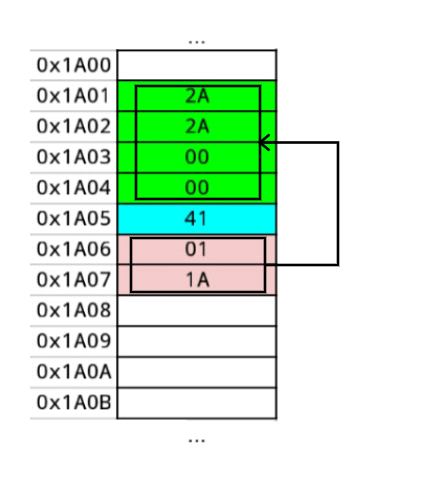
\includegraphics[height=0.60\textheight]{images/memptr}
    \end{columns}
\end{frame}

\begin{frame}
    \frametitle{Pointer Syntax}
    \begin{description}
        \item[Declaration]   {\em type} *{\em name}
            \par {\tt int *ptr;}
            \par Declares a pointer to a variable of given type.
        \item[Address Of]  \&{\em variable}
            \par {\tt \&x}
            \par Returns the address of the variable.
        \item[Dereference] *{\em name}
            \par {\tt *ptr}
            \par Gets to the value at the address stored in the pointer.
    \end{description}
\end{frame}

\begin{frame}[fragile]
    \frametitle{Pointer Example}
    \begin{verbatim}
int x;    //integer declaration
int *ptr; //integer pointer declaration

ptr = &x; //the "address of" operator
*ptr = 5; //dereferencing 
cout << ptr << endl;   //prints the address
cout << *ptr << endl;  //prints the value
    \end{verbatim}
    \begin{center}
       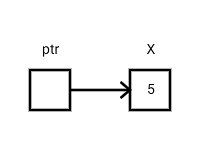
\includegraphics[height=0.25\textheight]{images/varptr}
    \end{center}
\end{frame}


\begin{frame}
    \frametitle{The {\tt new} and {\tt delete} Operators}
    \begin{block}{Syntax}
        \par{\tt new} {\em type}
        \par{\tt delete} {\em pointer}
    \end{block}
    \begin{itemize}
        \item {\tt new} allocates a new instance of the specified type.
        \item {\tt new} returns a pointer to the first byte of the newly 
            allocated memory.
        \item {\tt delete} deallocates the memory starting at the pointer.
        \item {\tt delete} only works on pointers returned by the {\tt new}
            operator.
    \end{itemize}
\end{frame}

\begin{frame}[fragile]
    \frametitle{Life of an Integer}
    \begin{verbatim}
int *ptr;

//create an integer
ptr = new int;

//do stuff with it
*ptr = 5;
cout << *ptr << endl;

//destroy it
delete ptr;
    \end{verbatim}
\end{frame}

\begin{frame}[fragile]
    \frametitle{Memory Leaks}
    \begin{columns}
        \column{0.5\textwidth}
        \begin{itemize}
            \item A very common bug!
            \item Memory leaks are when we have no reference to allocated
                memory.
            \item Allocated memory is effectively ``lost'' and becomes unusable.
            \item Wastes resources.
            \item In a loop, it can bring a system to its knees!
            \item Every {\tt new} should have a corresponding {\tt delete}
        \end{itemize}
        \column{0.5\textwidth}
        \begin{verbatim}
int *ptr;

ptr = new int;
ptr = nullptr;
//we lost an int!
        \end{verbatim}
    \end{columns}
\end{frame}

\begin{frame}
    \frametitle{Memory Organization}
    \begin{columns}
        \column{0.5\textwidth}
        \begin{itemize}
            \item Programs are usually divide into segments.
            \item A typical arrangement is based on the Unix Memory Model.
            \begin{itemize}
                \item Program Text
                \item Writable Data Block
                \item Program Stack
            \end{itemize}
            
        \end{itemize}
        
        \column{0.5\textwidth}
        \begin{center}
           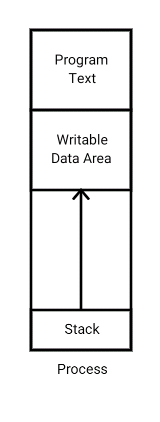
\includegraphics[height=0.8\textheight]{images/unixmem}
        \end{center}
    \end{columns}
\end{frame}

\begin{frame}
    \frametitle{Dynamic Memory}
    \begin{itemize}
        \item {\bf Static Variables} Variables declared normally.
        \item {\bf Dynamic Variables} Variables created with {\tt new}.
        \item A typical C++ arrangement:
        \begin{itemize}
            \item Static variables live on the stack.
            \item Dynamic variables live on the heap.
        \end{itemize}
        \item Static variables exist only while functions are running.
        \item Dynamic variables exist until deallocated.
    \end{itemize}
\end{frame}

\begin{frame}
    \frametitle{Arrays}
    \begin{itemize}
        \item Arrays are blocks of contiguous memory.
        \item They are a primitive list.
        \item Declared with type and size:
              \par {\tt int ar[10];}
        \item They are indexed, like vectors: {\tt ar[0]} thru {\tt ar[9]}
        \item Array bounds are immutable.
        \item Arrays are not objects!
        \item Typically, in C++, we use vectors.  Arrays just aren't as
            powerful!
    \end{itemize}
\end{frame}


\begin{frame}
    \frametitle{Arrays and Pointers}
    \begin{itemize}
        \item Like a pointer, an array name refers to a memory address.
        \item An array name is the address of the first item in the list.
        \item An array name can be assigned to a pointer!
            \par{\tt int *ptr = ar;}
        \item You can even index a pointer like an array (assuming it 
            contains the address of the beginning of an array)
            \par{\tt ptr[1]}
        \item Unlike pointers, array names are immutable.
        \item Arrays cannot be returned from functions while pointers can.
        \item More on the magic of pointers and arrays will be covered in
            your operating system class!
    \end{itemize}
\end{frame}


\begin{frame}
    \frametitle{Pointers and Objects}
    \begin{itemize}
        \item An object can be referenced by a pointer.
            \par{\tt Point *p;}
        \item You can create objects using {\tt new}:
            \par{\tt p = new Point; //invokes no-arg constructor}
            \par{\tt p = new Point(); //also no-arg}
            \par{\tt p = new Point(5,2); //arguments!}
        \item Members can be referenced using the {\tt ->} operator.
            \par{\tt p->setX(42.0);}
        \item Using {\tt delete} on an object invokes its destructor.
            \par{\tt delete p;}
    \end{itemize}
\end{frame}


\begin{frame}
    \frametitle{Advantages of Object Pointers}
    \begin{block}{Pro Tip}
        It is a very good idea to use pointers or references when
        dealing with objects!  Statically defined objects can be 
        trouble!
    \end{block}
    \begin{itemize}
        \item Explicit control of instantiation and destruction.
        \item Delay instantiation until some values have been computed.
        \item Pointers allow you to use {\tt nullptr} to indicate an
            object which has not yet been created.
        \item In C++, polymorphism only works with pointers and references!
    \end{itemize}
\end{frame}

\begin{frame}
    \frametitle{References Variables}
    \begin{itemize}
        \item Reference variables are declared with an {\tt \&}.
            \par{\tt Point p;}
            \par{\tt Point \&pref=p;}
        \item References bind the name to a memory location.
        \item References are immutable, and must be assigned at 
            instantiation.
    \end{itemize}
    \begin{block}{A Useful Idiom/Standard}
        Use pointers for creation and storage of objects.  Use
        references for parameters and non-dynamic member variables.
    \end{block}
\end{frame}

\section{Terminal Control}
\begin{frame}
    \frametitle{A Brief Introduction to TTY Interfaces}
    \begin{columns}
       \column{0.5\textwidth}
       \begin{itemize}
           \item Physical Hardware Terminals
           \item Linked to Machine via Serial Cables
           \item Video Terminals
           \item Type Writer (Teletype) Terminals
       \end{itemize}
       
       \column{0.5\textwidth}
       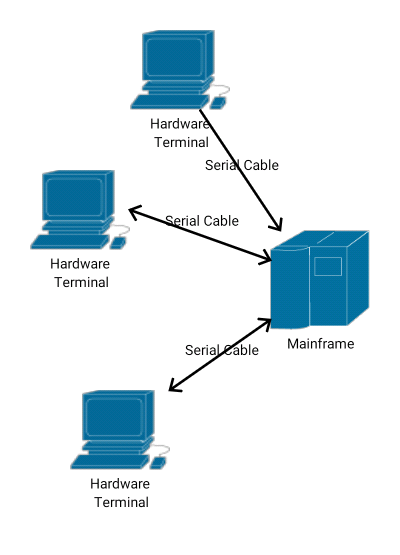
\includegraphics[width=\textwidth]{images/ttyoldschool}
    \end{columns}
\end{frame}

\begin{frame}
    \frametitle{Round Trip to Your Terminal}
    \begin{center}
        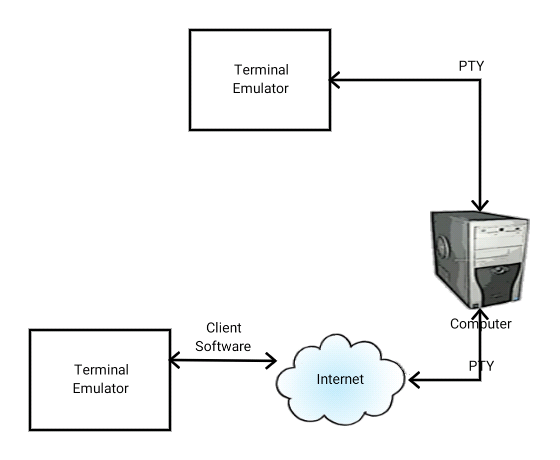
\includegraphics[height=0.8\textheight]{images/ttymodern}
    \end{center}
\end{frame}

\begin{frame}
    \frametitle{Terminal Control Codes}
    \begin{columns}
        \column{0.5\textwidth}
        \begin{itemize}
            \item Control uses Escape Sequences
            \item These begin with the escape character (octal 033)
            \item Sequences control color, cursor placement, etc.
            \item A terminal emulator responds to these sequences of characters.
        \end{itemize}
        
        \column{0.5\textwidth}
        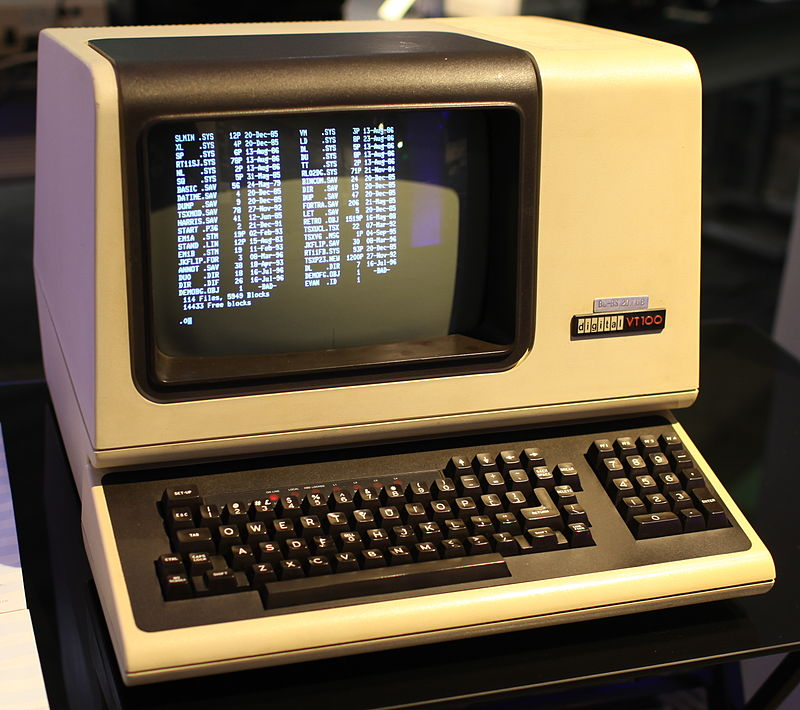
\includegraphics[width=\textwidth]{images/vt100}
        \imagesource{wikipedia.org}
    \end{columns}
\end{frame}

\begin{frame}
    \frametitle{termmanip.h}
    \begin{itemize}
        \item A small library written to play with terminals.
        \item It remembers the ANSI sequences so you don't have to!
        \item Works kind of like iomanip.  For instance example:
            \par{\tt cout << bold << red << "Hello, World" << endl;}
        \item Allows most common text changes and cursor movements.
    \end{itemize}
\end{frame}

\section{Conway's Game of Life}
\begin{frame}
    \frametitle{Cellular Automata}
    \begin{itemize}
        \item A simulation based on how cells reproduce.
        \item First CA's were proposed by John Von Neumann in the 1940's
        \item Many CA's are capable of Universal Computation!
        \item Useful in simulation problems, especially for optimization.
        \item Active area of research.
    \end{itemize}
\end{frame}

\begin{frame}
    \frametitle{The Rules of Conway's Game of Life}
    \begin{itemize}
    \item Proposed by John Conway in 1970
    \item Played on a 2D grid. 
    \item Each cell is either alive or dead.
    \item 4 Simple Rules:
    \begin{enumerate}
        \item {\bf Starvation} A living cell with fewer than 2 living         
            neighbors dies.
        \item {\bf Stasis} A living cell with 2-3 living neighbors lives.
        \item {\bf Overpopulation} A living cell with more than 3 living 
            neighbors dies.
        \item {\bf Reproduction} A dead cell with exactly two living 
           neighbors comes to life.
    \end{enumerate}
    \item Capable of Universal Computation!
    \end{itemize}
\end{frame}

\begin{frame}
    \frametitle{Some General Tips}
    \begin{itemize}
        \item Decompose the problem into classes.  Remember your parts of 
            speech!
        \item Each cell should basically just be aware of whether it is 
            alive or dead as well as whether it will be alive or dead in
            the next generation.
        \item A 2d grid can be represented as a vector of vectors:
            \par{\tt vector<vector<Cell> > grid(24, vector<Cell>(80));}
            \par{\tt grid[0][0];   //the upper left cell}
            \par{\tt grid[23][79]; //the lower right cell}
        \item The grid will need some way to count living neighbors.
    \end{itemize}
\end{frame}

\end{document}


